% Options for packages loaded elsewhere
\PassOptionsToPackage{unicode}{hyperref}
\PassOptionsToPackage{hyphens}{url}
%
\documentclass[
]{article}
\usepackage{amsmath,amssymb}
\usepackage{iftex}
\ifPDFTeX
  \usepackage[T1]{fontenc}
  \usepackage[utf8]{inputenc}
  \usepackage{textcomp} % provide euro and other symbols
\else % if luatex or xetex
  \usepackage{unicode-math} % this also loads fontspec
  \defaultfontfeatures{Scale=MatchLowercase}
  \defaultfontfeatures[\rmfamily]{Ligatures=TeX,Scale=1}
\fi
\usepackage{lmodern}
\ifPDFTeX\else
  % xetex/luatex font selection
\fi
% Use upquote if available, for straight quotes in verbatim environments
\IfFileExists{upquote.sty}{\usepackage{upquote}}{}
\IfFileExists{microtype.sty}{% use microtype if available
  \usepackage[]{microtype}
  \UseMicrotypeSet[protrusion]{basicmath} % disable protrusion for tt fonts
}{}
\makeatletter
\@ifundefined{KOMAClassName}{% if non-KOMA class
  \IfFileExists{parskip.sty}{%
    \usepackage{parskip}
  }{% else
    \setlength{\parindent}{0pt}
    \setlength{\parskip}{6pt plus 2pt minus 1pt}}
}{% if KOMA class
  \KOMAoptions{parskip=half}}
\makeatother
\usepackage{xcolor}
\usepackage[margin=1in]{geometry}
\usepackage{longtable,booktabs,array}
\usepackage{calc} % for calculating minipage widths
% Correct order of tables after \paragraph or \subparagraph
\usepackage{etoolbox}
\makeatletter
\patchcmd\longtable{\par}{\if@noskipsec\mbox{}\fi\par}{}{}
\makeatother
% Allow footnotes in longtable head/foot
\IfFileExists{footnotehyper.sty}{\usepackage{footnotehyper}}{\usepackage{footnote}}
\makesavenoteenv{longtable}
\usepackage{graphicx}
\makeatletter
\newsavebox\pandoc@box
\newcommand*\pandocbounded[1]{% scales image to fit in text height/width
  \sbox\pandoc@box{#1}%
  \Gscale@div\@tempa{\textheight}{\dimexpr\ht\pandoc@box+\dp\pandoc@box\relax}%
  \Gscale@div\@tempb{\linewidth}{\wd\pandoc@box}%
  \ifdim\@tempb\p@<\@tempa\p@\let\@tempa\@tempb\fi% select the smaller of both
  \ifdim\@tempa\p@<\p@\scalebox{\@tempa}{\usebox\pandoc@box}%
  \else\usebox{\pandoc@box}%
  \fi%
}
% Set default figure placement to htbp
\def\fps@figure{htbp}
\makeatother
\setlength{\emergencystretch}{3em} % prevent overfull lines
\providecommand{\tightlist}{%
  \setlength{\itemsep}{0pt}\setlength{\parskip}{0pt}}
\setcounter{secnumdepth}{5}
\usepackage{lineno}
% \linenumbers
\usepackage{float}
\usepackage[]{natbib}
\bibliographystyle{plainnat}
\usepackage{bookmark}
\IfFileExists{xurl.sty}{\usepackage{xurl}}{} % add URL line breaks if available
\urlstyle{same}
\hypersetup{
  pdftitle={Implications of Measurement Errors in Water Use Estimates for Water Management},
  pdfauthor={Taro Mieno; Timothy Foster; Nicholas Brozovic},
  hidelinks,
  pdfcreator={LaTeX via pandoc}}

\title{Implications of Measurement Errors in Water Use Estimates for Water Management}
\author{Taro Mieno\footnote{Department of Agricultural Economics, University of Nebraska Lincoln, \href{mailto:tmieno2@unl.edu}{\nolinkurl{tmieno2@unl.edu}}} \and Timothy Foster\footnote{Department of WWW, University of Manchester, \href{mailto:timothy.foster@manchester.ac.uk}{\nolinkurl{timothy.foster@manchester.ac.uk}}} \and Nicholas Brozovic\footnote{Department of Agricultural Economics, University of Nebraska Lincoln, \href{mailto:nbrozovic@nebraska.edu}{\nolinkurl{nbrozovic@nebraska.edu}}}}
\date{}

\begin{document}
\maketitle
\begin{abstract}
abstract here
\end{abstract}

\newpage

\section{Main}\label{main}

\subsection{Background}\label{background}

\begin{itemize}
\item
  intensity estimation accuracy
\item
  (estimated) intensity-based vs (estimated) area-based (Southern Europe History)
\item
  (estimated) intensity-based vs (true) intensity-based {[}We work on this{]}
\item
  Lack of measurement. Use of water use estimates for water management (current and future). Emergence of Open ET as a substitute.
\end{itemize}

key objective:

\begin{itemize}
\item
  start a discussion about the implications of the use of mis-measured water use for water use regulation.
\item
  shed lights on unintentional consequences of using estiamtes rather than actual measurements
\end{itemize}

Two policies:

\begin{itemize}
\tightlist
\item
  water quota (examples of existing quota systems)
\item
  water permit trading
\end{itemize}

No clear policy design suggestions on how to use water use estiamtes with measurement errors.

\section{Results}\label{results}

\subsection{Profit under water and proxy quota}\label{profit-under-water-and-proxy-quota}

Figure \ref{fig:profit-quota-water-het} below compares profit from agricultural production as a function of actual water use between water and proxy quota across three different production heterogeneity levels and the size of the measurement errors. When there is no heterogeneity in farmers' production function, water quota is the most cost effective way to achieve a water use reduction goal (highest profit achievable for a given level of actual water use). Under this circumstance, proxy quota with unbiased measurement errors achieves worse than water quota due to asymmetry in downside and upside risk of water use. However, as production heterogeneity increases, water quota loses its comparative advantage over proxy quota. It can be shown that water quota always outperforms proxy quota on average irrespective of the degere of production heterogeneity when measurement error is independent and production function is concave (show proof in appendix). Not surprisingly, profit losses of using proxy quota increase as measurement error size increases. Profit loss of using proxy-based quota tends to become greater as the toal realized water use becomes smaller.

\begin{figure}[H]

{\centering 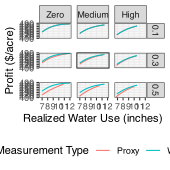
\includegraphics{figures/g_profit_quota_comp_stat} 

}

\caption{The impacts of an increase in the degree of measurement error on profit}\label{fig:profit-quota-water-het}
\end{figure}

We now look at simple two-farm examles to build intuition behind the profit loss due to the use of proxy quota in place of water quota. Figure \ref{fig:illust-homegeneous} presents a case with two homegeneous farmers under water and proxy quota. The red dotted lines indicate the effective water quota. Under the water quota system, both farmers receive 7 inches of water quota. Since the unconstrained profit maximizing water use is 10.94 inches, both farmers use up all the allocated quota and use 10 inches of water. Under the proxy quota system, they are allocated the same amount of proxy quota. However, measurement error in proxy quota resulted in effective water quota of 4 and 10 inches for farmer A and B, respectively. Both farmers use their allocated amout of water. Under both proxy and water quota systems, the total water use is 14 inches. Farmer B makes 29.9 less under the water quota system compared to the proxy quota system. However, Farmer A makes 128.9 more under the water quota system compared to the proxy quota system. This comes from an important nature of crop production with respsect to water: declining marginal impact of water on crop yield. As can be seen in the profit-water relationship, removing an inch of water from 6 inches has much larger negative impact compared to revmoing an inch of water from 10 inches.

\begin{figure}[H]

{\centering \includegraphics{figures/g_illustration_homogeneous} 

}

\caption{Illustration of profit loss due to the use of proxy for quota-based regulation: a case of homegeneous producers}\label{fig:illust-homegeneous}
\end{figure}

However, as the heterogeneity of farmers increases, comparative advantage of water quota over proxy quota diminishes. While the performance of both systems declines as the level of heterogeneity increases, water quota is affected more so than the proxy quota system. This is because uniform quota now acts like heterogeneous quota under homogeneous production function because the same quota is given to farmers with heterogeneous water demand. This is illustrated in Figure \ref{fig:illust-heterogeneous}. In this example, farmer A needs less water than farmer B. Water and proxy quota allocated to the farmers are exactly the same as the previous case. In this example, errors in proxy happened to realize so that more effective water quota is given to farmer B than farmer A. Consequently, proxy quota produces a higher total profit than water quota. Of course, if error happened to go the opposite way, then the performance of proxy quota relative to water quota is even worse compared to the homogeneous case. This is a big contrast to the homogeneous case because water quota is always better than proxy quota in that case. Consequently, proxy quota performs relatively better under heterogeneous cases. On average, the positive and negative effects of measurement errors tend to even out. However, proxy quota is never better than water quota \textbf{on average} (see Appendix \ldots{} for mathematical proof).

\begin{figure}[H]

{\centering \includegraphics{figures/g_illustration_het} 

}

\caption{Illustration of profit loss due to the use of proxy for quota-based regulation: a case of heterogeneous producers}\label{fig:illust-heterogeneous}
\end{figure}

\textbf{Convert $u\_dev$ to $R^2$.}

\subsection{The effect of allowing trading quota}\label{the-effect-of-allowing-trading-quota}

Allowing quota to be traded among farmers can dramatically change the relative performance of the water- and quota-based regulation. Figure \ref{fig:trading-profit} presents profit for water-based quota, proxy-based quota, water-based quota trading, and proxy-based quota trading regulation systems. As shown in the figure, the disadvantage of using proxy almost disappears when trading of quota is allowed. This is because the inefficiencies in quota allocations are resolved through trading of quota whether it is water or proxy quota.

\begin{figure}[H]

{\centering \includegraphics{figures/g_trade_effect_profit} 

}

\caption{Comparison of profit from agricultural production between the water and quota systems when quota trading is allowed}\label{fig:trading-profit}
\end{figure}

Figure \ref{fig:trading-profit-illustration} illustrates the impact of allowing for trading proxy quota using the case of two homogeneous farmers illustrated in Figure \ref{fig:illust-homegeneous}. In this illustration, the same water quota of 7 is allocated for both farmers under the water-based systems. No water quota trading would happen as the marginal profit of water is already equated at water use of 7. Under the proxy-base quota system, proxy quota of 7 is allocated for both farmers, but the effective water quota for farmers A and B are 4 and 7, respectively. Once trading of proxy quota is alllowed, farmer A would buy 1.85 proxy quota from farmer B. At these production levels, the marginal profit of quota (not water) are equated acros the farmers and no further transfer between them would happen. Trading of proxy quota improves the overall profit to 920.08 \$/acre from 831.94 \$/acre.

\begin{figure}[H]

{\centering \includegraphics{figures/g_illustration_homogeneous_with_trade} 

}

\caption{Illustration of the benefits of trading quota}\label{fig:trading-profit-illustration}
\end{figure}

While water-quota and proxy-quota trading perform about the same, water-quota always leads to a higher total profit for a given level of realized water use. In other words, to achieve a certain water use goal, water-quota trading is always to more cost-effective than proxy-quota trading. Under water-quota trading, the margial profit of water is equalized across the farmers, which is a necessary condition to achieve the highest profit for a given level of total water use. Under proxy-quota trading, the marginal profit of proxy is equalized across the farmers, not the margial profit of water (See Appendix \ldots{} for a mathematical proof). However, it is worth emphasizing that the inefficiency caused by the use of proxy is likely to be minimal as shown in Figure \ref{fig:trading-profit}. This point is well-illustrated in Figure \ref{fig:trading-profit-illustration}, where total profit per acre is 930.91 and 920.08 under the water-quota and proxy-quota trading system, respsectively.

Figure \ref{fig:trading-profit} presents the simualtion results of proxy-quota and water-quota trading systems added to Figure \ref{fig:profit-quota-water-het}. As you can see at all levels of production heterogeneity levels and the degres of measurement errors, proxy-quota and water-quota trading systems perform almost identical at all levels of realized water use (water-quota trading is always slightly better than proxy-quota trading as explained earlier). Not surprisingly, the benefit of allowing for trading is greater when the degree of measurement errors is larger.

\subsection{Use of proxy can exercebate distributional inequity}\label{use-of-proxy-can-exercebate-distributional-inequity}

Figure \ref{fig:distributional-equity} presents the cumulative probability of the ratio of profit under quota-based relative to water-based system for quota (red) and permit trading (blue). Ratio of less than 1 indicates making less profit under the quota-based system compared to the water-based system. If farmers make just as much profir under proxy-based regulation compared to water-based regulation, then the cumulative probability line would be a vertical line at 1. For example, under the high degree of measurement error and medium heterogenenity scenario, some farmers would make about the half of what they would make under the water quota system. At the lower end of the distribution are farmers who would be constrained severely by water quota, but whose water use estiamtes are much higher than their actual water use. At the higher end of the distribution are farmers who would be constrained by water quota, but whose water use estiamtes are much lower than their actual water use. Famres who suffer significantly under the quota system can develop strong dissatisfaction of the quota-based regulation system, which in turn may lead to installing water meter themselves. If they discover the over-estimation of their water use, they may appeal to legal actions against the administrator for their unfair treatment. Allowind quota trading greatly diminishes the distributional inequality, though not completely. This is because unfortunate farmers who suffered from over-estimation of their water use can now at least purchase proxy quota to increase their production level.

\begin{figure}[H]

{\centering \includegraphics{figures/g_profit_ratio} 

}

\caption{Distribution of profit under various regulation systems}\label{fig:distributional-equity}
\end{figure}

\section{Discussion}\label{discussion}

\begin{itemize}
\tightlist
\item
  Unbiased proxy

  \begin{itemize}
  \tightlist
  \item
    can hurt profit\\
  \item
    elements that matter

    \begin{itemize}
    \tightlist
    \item
      the heterogeneity of production function
    \item
      the degree of measurement error
    \end{itemize}
  \end{itemize}
\item
  Allowing quota trading can be particularly beneficial when proxy is used.

  \begin{itemize}
  \tightlist
  \item
    Trade-off of implementing quota trading (this is not anything new)

    \begin{itemize}
    \tightlist
    \item
      gain in profit from agricultural production
    \item
      administrative cost
    \end{itemize}
  \end{itemize}
\item
  Use of proxy exercebates distributional inequality

  \begin{itemize}
  \tightlist
  \item
    trading quota can help here again
  \item
    greater chance of litigations from farmers against the administrator
  \end{itemize}
\item
  Limitations

  \begin{itemize}
  \tightlist
  \item
    Assumptions (farmers have linked their practice and water use estimates, but not water)

    \begin{itemize}
    \tightlist
    \item
      uncertainty in water use estimates lead to under-use of water, harming profit even more
    \end{itemize}
  \item
    Temporal

    \begin{itemize}
    \tightlist
    \item
      one-year decision
    \item
      other quota designs (multiple year)
    \end{itemize}
  \end{itemize}
\end{itemize}

\section{Methods}\label{methods}

This section describes the details of the simulation analysis conducted in this article. Our simulation imagines a region with 1000 (denoted as \(N\), hereafter) farmers, where a single water governing body possesses a right to devise groundwater policies. Our simulation considers nine scenarios in total: three different levels of production heterogeneity times three different degrees of measurement errors. Under each scenario, 1000 rounds of individual simulations are run. In each simulation round, measurement errors are drawn randomly for the individual farmers, and then average (across the farmers) water use and profit are calculated at different levels of water or proxy quota levels for four different policies: water-quota, proxy-quota, water-quota trading, proxy-quota trading. The summary of the 1000 simulation rounds. The key components of the simluation analysis are presented below.

\subsection{Crop-water production function}\label{crop-water-production-function}

For all faemers \(i \in 1,\dots, N\), the crop-water production function follows the Michelich-Baule functional form presented below(citations).

\begin{equation}
y_i = f_i(w) = \phi_i (1 - \alpha_i \cdot e^{-\beta_i\cdot w})
\end{equation}

where \(y\) is corn yield (kg/ha), \(w\) is water use (mm), and \(\phi\), \(\alpha\), and \(\beta\) are model parameters that govern how corn yield responds to water use.

Given the price of corn (\(P_c\)) and water (\(P_w\)), farmer \(i\) is assumed to maximize profit by solving the following maximization problem when no water quota is placed:

\begin{equation}
w^* = argmax_{w} \;\; P_c \cdot f_i(w) - P_w \cdot w
\end{equation}

Three different sets of the collections of crop-water production functions are generated that vary in the degree of heterogeneity in unconstrained optimal water use (\(w^*\)). Under no-heterogeneity set, farmers share exactly the same profuction function (the same value of \(\phi_i\), \(\alpha_i\), and \(\beta_i\)). Unde the medium-heterogeneity set, model parameters vary and so does \(w^*\). Under the high-heterogeneity set, the variance of \(w^*\) becomes even greater. The distribution of \(w^*\) for each of the sets is presented in Figure \ref{fig:dist-opt-w}.

\subsection{Measurement error in water use}\label{measurement-error-in-water-use}

When water use values are not measured and observed, the administrator estimates water use. The estimated value of water use is named ``proxy'' and denoted as \(p\). Proxy and water are assumed to follow the relationship below for all the farmers (\(i \in 1,\dots, N\)):

\begin{equation}
p = \eta_i \cdot w
\end{equation}

where \(\eta_i\) is a scalar greater than 0. Measurement error (denoted as \(\mu\)) can be written as follows:

\begin{equation}
\mu_i = p - w = (\eta_i - 1)\cdot w
\end{equation}

While farmers with \(\eta_i > 1\) are unfortunate and their water uses are over-estimated, farmers with \(\eta_i < 1\) are fortunate and their water uses are under-estimated.

Three different sets of the distribution of \(\eta\) are considered that vary in the degree of heterogeneity in \(\eta\): low, medium, and high. For all the sets, \(E[\eta] = 1\) (or equivalently \(E[\mu] = 0\)), meaning that water use estimation is ubiased. A sample of the empirical (realized) distribution of \(\eta\) for each of the sets is presented in Figure \ref{fig:dist-eta}.

\subsection{Water use under quota and trading systems}\label{water-use-under-quota-and-trading-systems}

Under both water and proxy quota systems without trading, the same amount of quota is allocated to all the farmers. (this is realistic with insufficient information available to the administrator). For a given water quota of \(\overline{w}\), farmer \(i\)'s water use would be \(min\{w^*, \overline{w}\}\). Under the proxy quota system, the same amount of proxy quota (\(\overline{p}\)) is allocated to all the farmers. However, the effective limit on water use varies by farmer. Given the proxy quota of \(\overline{p}\), the effective water use limit for farmer \(i\) is \(\overline{p} / \eta_i\), and uses \(min\{w^*, \overline{p} / \eta_i\}\).

Assumptions:
+ farmers: has learned the degree of under- or over-estimation of water use compared to actual over the years and has learned how to irrigate up to the water quota

Under a water trading system, the same amount of water quota is first allocated to all the farmers just like water quota system. However, farmers are now allowed to sell or buy water quota under a water trading system. Assuming no transaction cost of trading, water quota will be traded until the marginal profit of water at their respective level of water uses is equated across the farmers. Let \(\pi_i(w)\) denote farmer \(i\)'s profit: \(P_c \cdot f_i(w) - P_w \cdot w\). Conditional on water quota of \(\overline{w}\), individual water uses for the farmers can be identified by finding a series of water use values (\(w_1, w_2, \dots, w_N\)) that satisfy the following conditions:

\begin{align}
& \frac{\partial \pi_1(w)}{\partial w}\Big\rvert_{w = w_1} = \frac{\partial \pi_2(w)}{\partial w}\Big\rvert_{w = w_2} = \dots = \frac{\partial \pi_N(w)}{\partial w}\Big\rvert_{w = w_N} \\
& \sum_{i=1}^N w_i = N \cdot \overline{w}
\end{align}

Under a proxy trading system, proxy quota will be traded until the marginal profit of proxy (not water) at their respective level of effective water (or equivalently proxy) uses is equated across the farmers. Conditional on proxy quota of \(\overline{p}\), individual proxy use for the farmers can be identified by finding a series of proxy use values (\(p_1, p_2, \dots, p_N\)) that satisfy the following conditions:

\begin{align}
& \frac{\partial \pi_1(w)}{\partial p}\Big\rvert_{p = p_1} = \frac{\partial \pi_2(w)}{\partial p}\Big\rvert_{p = p_2} = \dots = \frac{\partial \pi_N(w)}{\partial p}\Big\rvert_{p = p_N} \\
& \sum_{i=1}^N p_i = N \cdot \overline{p}
\end{align}

\subsection{Data and Code Availability}\label{data-and-code-availability}

The datasets created in this article are all computer-generated using R codes. All the datasets and codes are available at the \href{https://github.com/tmieno2/Measurement-Error-Water-Management}{following GitHub repository}.

\clearpage

\appendix


\subsection{Distribution of optimal water use under no water use constraints}\label{distribution-of-optimal-water-use-under-no-water-use-constraints}

\begin{figure}[H]

{\centering \includegraphics{figures/g_opt_w_dist} 

}

\caption{Distribution of optimal water use under no water use constraints}\label{fig:dist-opt-w}
\end{figure}

\subsection{Distribution of water-proxy conversion factor}\label{distribution-of-water-proxy-conversion-factor}

\clearpage

  \bibliography{DRA.bib}

\end{document}
